\documentclass[12pt]{article}
\usepackage{amsmath, amssymb, enumitem, fancyhdr, graphicx, libertine, nth,
  pgfplots, tikz, xcolor}
\pgfplotsset{compat=1.11}
\usepackage[margin=1in]{geometry}
\usepackage[libertine]{newtxmath}
\definecolor{solution-color}{HTML}{000080}

\pagestyle{fancy}
\chead{\emph{EC201 -- Problem Set 1 -- Solutions}}

% Define new topic command
\newcommand{\topic}[1]{\begin{center}\large\textsc{#1}\normalsize\end{center}}

% Define question counter:
\newcounter{question}[section]
\newcommand{\question}[1]{\refstepcounter{question}
  \subsubsection*{Question~\thequestion~-- #1}}

% Subquestions are enumerate with letters
\newenvironment{subquestions}{
  \begin{enumerate}[label=(\roman*)]}{\end{enumerate}}

\begin{document}

\topic{Mathematics Review}

\question{Differentiation}
Differentiate the following functions, i.e.~find $\frac{df\left( x
\right)}{dx}$:
\begin{subquestions}
  \item $f\left( x \right)= 4x^2$
    \textcolor{solution-color}{
      \[
        \frac{df\left( x \right)}{dx} = 8x
      \]
    }
  \item $f\left( x \right)= 201$ \\
    \textcolor{solution-color}{
      The derivative of a constant is zero:
      \[
        \frac{df\left( x \right)}{dx} = 0
      \]
    }
  \item $f\left( x \right)= 2x + 4x^3$
    \textcolor{solution-color}{
      \[
        \frac{df\left( x \right)}{dx} = 2 + 12x^2
      \]
    }
\end{subquestions}

\question{Partial Differentiation}
Find the partial derivatives of the following functions, i.e.~find
$\frac{\partial f\left( x_1,x_2 \right)}{\partial x_1}$ and
$\frac{\partial f\left( x_1,x_2 \right)}{\partial x_2}$:
\begin{subquestions}
  \item $f\left( x_1,x_2 \right)=x_1^{\frac{1}{3}}x_2^{\frac{2}{3}}$

    \textcolor{solution-color}{
      When we take the partial derivative of the function with respect to $x_1$,
      we treat $x_2$ as if it were a constant. Since the $x_2$ term is
      \emph{multiplied} by the $x_1$ term, we just leave it there as it is:
      \[
        \frac{\partial f\left( x_1,x_2 \right)}{dx_1}
        =\frac{1}{3}x_1^{\frac{1}{3}-1}x_2^{\frac{2}{3}}
        =\frac{1}{3}x_1^{-\frac{2}{3}}x_2^{\frac{2}{3}}
      \]
      For $x_2$ we follow the same approach:
      \[
        \frac{\partial f\left( x_1,x_2 \right)}{dx_2}
        =\frac{2}{3}x_1^{\frac{1}{3}}x_2^{\frac{2}{3}-1}
        =\frac{2}{3}x_1^{\frac{1}{3}}x_2^{-\frac{1}{3}}
      \]
    }
  \item $f\left( x_1,x_2 \right)=2x_1 + 3x_2^2$

    \textcolor{solution-color}{
      When we take the partial derivative of the function with respect to
      $x_1$, we treat $x_2$ as a constant. Since the $x_2$ term is \emph{not
      multiplied} by the $x_1$ term, it drops out when we take the partial
      derivative (because the derivative of just a constant is zero):
      \[
        \frac{\partial f\left( x_1,x_2 \right)}{dx_1} = 2
      \]
      Similarly when we hold $x_1$ constant:
      \[
        \frac{\partial f\left( x_1,x_2 \right)}{dx_2} = 6x_2
      \]
    }

\end{subquestions}

\question{Optimization}
For each of the functions below, do the following:
\begin{itemize}
  \item Sketch the graph of the function.
  \item Find $\frac{df\left( x \right)}{dx}$
  \item Find the extreme point, i.e.~at what $x^{\star}$ is $\frac{df\left(
    x^{\star} \right)}{dx}=0$?
  \item Is the extreme point a maximum or a minimum? (To do this you will need
    to find the second derivative.)
\end{itemize}
\begin{subquestions}
  \item $f\left( x \right) = 8x - 2x^2$

      \textcolor{solution-color}{
        Here is the function displayed as a graph: \\
        \begin{center}
          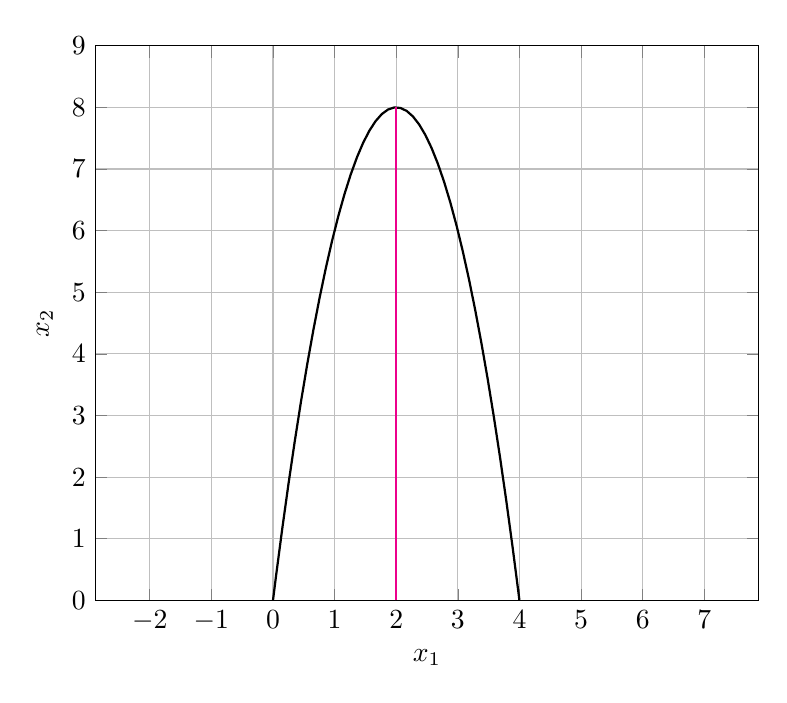
\begin{tikzpicture}[baseline]
            \begin{axis}[axis equal,
                         grid=both,
                         xmax=5,xmin=0,
                         ymin=0,ymax=9,
                         xlabel=$x_1$,ylabel=$x_2$,
                         xtick={-2,...,8},
                         ytick={-1,...,9},
                         width=10cm,
                         anchor=center]
              \addplot[thick, samples=100] {-2*x^2+8*x};
              \addplot[thick, magenta] coordinates {(2,0)(2,8)};
            \end{axis}
          \end{tikzpicture}
        \end{center}
        The derivative is:
        \[\frac{df\left( x \right)}{dx}=8 - 4x \]
        The extreme point happens when $\frac{df\left( x \right)}{dx}=0$
        So:
        \[
          8 - 4x^\star =0 \Rightarrow x^\star = \frac{8}{4} = 2
        \]
        From the graph we can see that this is a maximum. However we can also
        use the second derivative to check if it is a maximum or a minimum. The
        second derivative is:
        \[\frac{d^2f\left( x \right)}{dx^2}=- 4 \]
        When the second derivative is negative, we know that it is a maximum.
      }
  \item $f\left( x \right) = x^2$

    \textcolor{solution-color}{
      Here is the function displayed as a graph: \\
      \begin{center}
        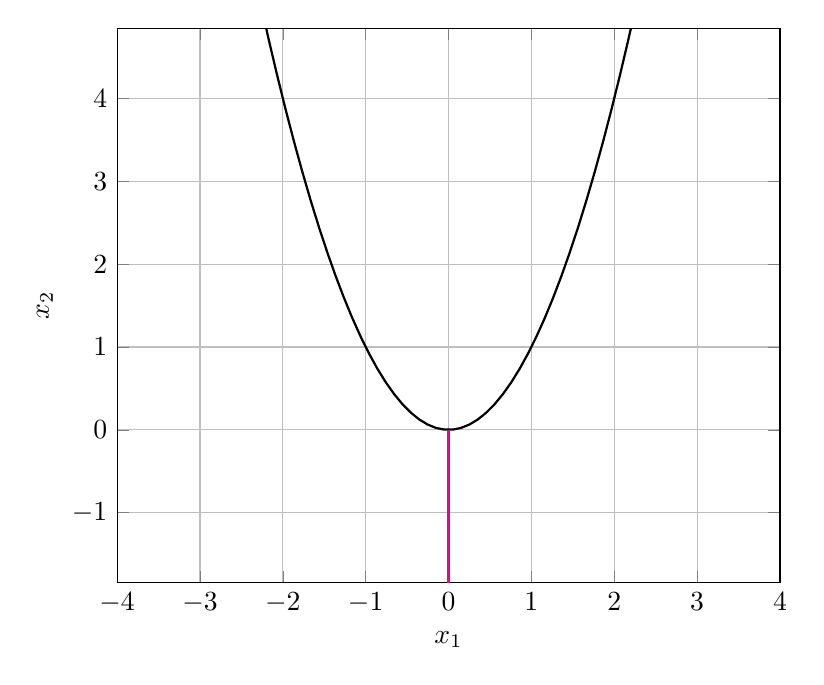
\begin{tikzpicture}[baseline]
          \begin{axis}[axis equal,
                       grid=both,
                       xmax=4,xmin=0-4,
                       ymin=-1,ymax=4,
                       xlabel=$x_1$,ylabel=$x_2$,
                       xtick={-4,...,4},
                       ytick={-1,...,4},
                       width=10cm,
                       anchor=center]
            \addplot[thick, samples=100] {x^2};
            \addplot[thick, magenta] coordinates {(0,-2)(0,0)};
          \end{axis}
        \end{tikzpicture}
      \end{center}
      The derivative is
      \[\frac{df\left( x \right)}{dx}= 2x\]
      $\frac{df\left( x \right)}{dx}$ is zero when $x=0$ so $x^\star = 0$.
      From the graph we can see that this is a minimum. The second
      derivative is:
      \[\frac{d^2f\left( x \right)}{dx^2}= 2 \]
      Since this is positive, we know that it is a minimum.
    }
\end{subquestions}

\topic{The Budget Constraint}
\question{Two Price Changes}
An individual's budget line is given by:
\[
  p_1x_1 + p_2x_2 = m
\]
Suppose the price of good 1 doubled and the price of good 2 halved.
Sketch the original and new budget constraints.

\textcolor{solution-color}{
  We saw in class that we can isolate $x_2$ on the left-hand side to write the
  budget constraint as
  \[
    x_2 =\frac{m}{p_2} - \frac{p_1}{p_2}x_1
  \]
  Thus the vertical intercept is at $\frac{m}{p_2}$ and the slope is
  $-\frac{p_1}{p_2}$. With the change in prices, the budget constraint becomes:
  \[
    2p_1x_1 + \frac{1}{2}p_2x_2 =m
  \]
  Rewriting this with $x_2$ isolated on the left-hand side is:
  \begin{align*}
    \frac{1}{2}p_2 x_2 &= m - 2p_1x_1\\
    x_2 &= \frac{2m}{p_2} - \frac{4p_1}{p_2}x_1
  \end{align*}
  Thus the vertial intercept is now twice as high ($\frac{2m}{p_2}$ versus
  $\frac{m}{p_2}$) and the slope is four times as steep ($-\frac{4p_1}{p_2}$ versus
  $-\frac{p_1}{p_2}$).
  The old and new budget lines are graphed below.
  \begin{center}
    \begin{tikzpicture}[baseline]
      \begin{axis}[axis equal,
                   ticks=none,
                   xmax=3,xmin=0,
                   ymin=-1,ymax=5,
                   xlabel=$x_1$,ylabel=$x_2$,
                   domain = 0:4,
                   axis x line = middle,
                   axis y line = middle,
                   width=10cm,
                   anchor=center]
        \addplot[samples=1000, restrict y to domain = 0:4] {2 - x};
        \addplot[dashed, magenta, samples=50, restrict y to domain = 0:4] {4 -
        4 * x};
        \draw (0, 2) node [left] {$\frac{m}{p_2}$};
        \draw (0, 4) node [magenta, left] {$\frac{2m}{p_2}$};
        \draw (1, 0) node [magenta, below] {$\frac{m}{2p_1}$};
        \draw (2, 0) node [below] {$\frac{m}{p_1}$};
        \draw (0.4, 3) node [magenta, right] {Slope: $-\frac{4p_1}{p_2}$};
        \draw (1.4, 0.8) node [right] {Slope: $-\frac{p_1}{p_2}$};
      \end{axis}
    \end{tikzpicture}
  \end{center}
  The old budget line is the solid line and the new budget line is the dashed
  line.
}

\question{Price and Income Changes}
Suppose next year the prices of goods 1 and 2 will
increase by 5\% and your salary will also increase by 5\%. Describe how this
affects your budget line.

\textcolor{solution-color}{
  If all prices and income change by the same amount, the budget line will not
  change at all. To see this, start off with the original budget line:
  \[
    p_1x_1 + p_2x_2 =m
  \]
  Now let's increase prices and income by 5\%. This is like multiplying prices
  and income by 1.05:
  \[
    1.05 p_1x_1 + 1.05 p_2x_2 =1.05 m
  \]
  If we divide both sides of the equation by 1.05, we end up with the original
  budget line:
  \[
    p_1x_1 + p_2x_2 =m
  \]
  Thus increasing all prices and income by the same amount does not affect the
  budget line.
}

\newpage
\topic{Preferences}
\question{Indifference Curves}
Suppose you enjoy consuming good 1 but you are not at all interested in good 2 (you are neutral about good 2). If you ever get any of good 2 you just give it away.  What would your indifference curves look like? Sketch them.

\textcolor{solution-color}{
  Suppose we fix the amount of $x_1$ that you have (the good that you enjoy consuming). If we give you any more or less of $x_2$ (the good that you don't like), it will not change your utility. You are indifferent between any bundles that have more or less of $x_2$ as long as they have the same amount of $x_1$.
}

\textcolor{solution-color}{
  For example, suppose we started out with the bundle $\left( 1,1 \right)$. You
  have one of good 1 and one of good 2. We want to try and find bundles that
  you would be indifferent to.
  \begin{itemize}
    \item $\left( 1,0 \right)$ is one such bundle. You have the same amount of good 1 as before (the good that you like) but you no longer have any good 2. You are indifferent between $\left( 1,1 \right)$ and $\left( 1,0 \right)$ because you we were going to give away any $x_2$ that you had anyway, so if you don't have any it's the same as having 1 unit.
    \item $\left( 1,2 \right)$ is another such bundle. You have the same amount
      of good 1 as before but you have extra good 2. Since you give away any good 2
      it doesn't give you any extra utility. Hence you are
      indifferent.
    \item $\left( 1,10 \right)$ is another bundle. It really doesn't matter how
      much $x_2$ you get as long as you have the same amount of $x_1$. You will
      always throw good 2 away.
  \end{itemize}
  The pattern here is that it doesn't matter how much $x_2$ you have as long as
  you have the same amount of good 1. Indifference curves are therefore vertical
  lines like this:
}
\textcolor{solution-color}{
  \begin{center}
    \begin{tikzpicture}[baseline]
      \begin{axis}[axis equal,
                   ticks=none,
                   xmax=5,xmin=0,
                   ymin=0,ymax=3,
                   xlabel=$x_1$,ylabel=$x_2$,
                   domain = 0:4,
                   axis x line = middle,
                   axis y line = middle,
                   width=10cm,
                   anchor=center]
        \addplot[thick] coordinates {(1,0)(1,3)};
        \addplot[thick] coordinates {(2,0)(2,3)};
        \addplot[thick] coordinates {(3,0)(3,3)};
        \addplot[thick] coordinates {(4,0)(4,3)};
      \end{axis}
    \end{tikzpicture}
  \end{center}
}

\newpage
\topic{Utility}
\question{Indifference Curves and the Marginal Rate of Substitution}
Answer the following questions about these utility functions:
\begin{subquestions}
  \item $u\left(x_1, x_2  \right)=x_1 + 2x_2$.
    \begin{itemize}
      \item Sketch the indifference curves of the utility function for
        fixed levels of utility $k=1$, $k=2$ and $k=3$.

        \textcolor{solution-color}{
          We start with setting utility equal to $k$ and then solving for $x_2$:
          \begin{align*}
            k &= x_1 + 2x_2 \\
            x_2 &= \frac{k}{2} - \frac{1}{2}x_1
          \end{align*}
          Now for $k=1$, $k=2$ and $k=3$ we draw the lines:
          \begin{center}
            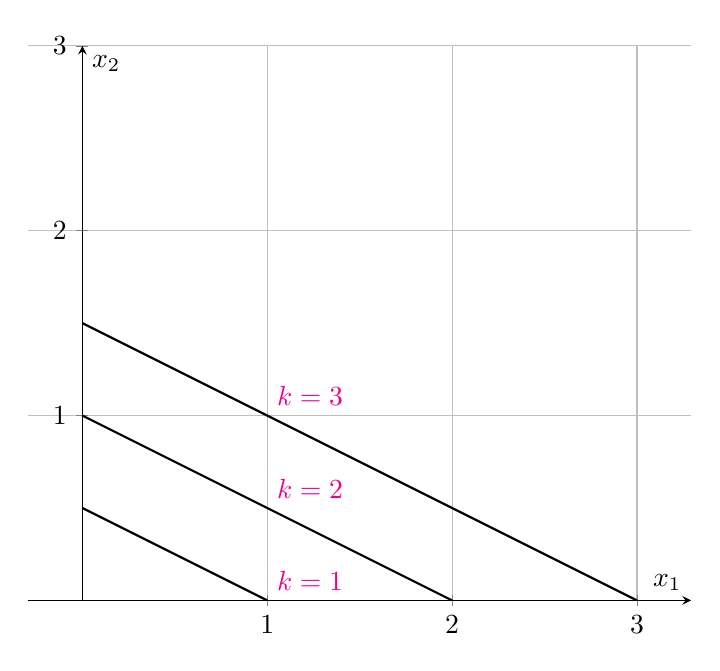
\begin{tikzpicture}[baseline]
              \begin{axis}[axis equal,
                           axis x line = middle,
                           axis y line = middle,
                           grid=both,
                           xmax=3,xmin=0,
                           ymin=0,ymax=3,
                           xlabel=$x_1$,ylabel=$x_2$,
                           xtick={0,...,3},
                           ytick={0,...,3},
                           width=10cm,
                           anchor=center]
                \addplot[thick] coordinates {(0,0.5)(1,0)};
                \addplot[thick] coordinates {(0,1)(2,0)};
                \addplot[thick] coordinates {(0,1.5)(3,0)};
                \draw (1, 1) node [magenta, above right] {$k=3$};
                \draw (1, 0.5) node [magenta, above right] {$k=2$};
                \draw (1, 0) node [magenta, above right] {$k=1$};
              \end{axis}
            \end{tikzpicture}
          \end{center}
        }
      \item Calculate the marginal rate of substitution ($MRS$) between the two
        goods, where: \[ MRS = -\frac{\frac{\partial u\left( x_1,x_2
        \right)}{\partial x_1}}{\frac{\partial u\left( x_1,x_2
      \right)}{\partial x_2}} \]
        \textcolor{solution-color}{
          The marginal utility from $x_1$ is $\frac{\partial u\left( x_1,x_2
          \right)}{\partial x_1}=1$ and
          the marginal utility from $x_2$ is $\frac{\partial u\left( x_1,x_2
          \right)}{\partial x_2}=2$. The marginal rate of substitution is then:
          \[
            MRS=-\frac{1}{2}
          \]
          This is precisely the slope of the indifference curves.
        }
      \item Can you come up with an example of two goods where this
      utility function would be reasonable?

        \textcolor{solution-color}{
          An example of two ``goods'' that could satisfy these preferences are
          \$5 and \$10 bills. A \$10 bill would normally give people twice the
          utility as a \$5 bill (or you are indifferent between 2 \$5 bills and
          one \$10 bill). So $x_1$ could be a \$5 bill and $x_2$ could
          be a \$10 bill.
        }
    \end{itemize}
  \item $u\left( x_1,x_2 \right)=\min\left\{\frac{1}{2}x_1, x_2\right\}$
    \begin{itemize}
      \item Sketch the indifference curves of the utility function for
        fixed levels of utility $k=1$, $k=2$ and $k=3$.

        \textcolor{solution-color}{
          If we set utility to $k$ we get:
          \[
            k = \min\left\{\frac{1}{2}x_1, x_2\right\}
          \]
          \begin{itemize}
            \item If $x_2\leq \frac{1}{2}x_1$, then this is the same as
              $k=x_2$, so solving for $x_2$ is just $x_2 = k$.
            \item If $x_2>\frac{1}{2}x_1$, then $x_2$ can be any
              number at all, provided it's at least $\frac{1}{2}x_1$.
          \end{itemize}
          At the kink points we have $\frac{1}{2}x_1=x_2$ so $x_1$ needs to be
          double $x_2$. Drawing the indifference curves gives:
          \begin{center}
            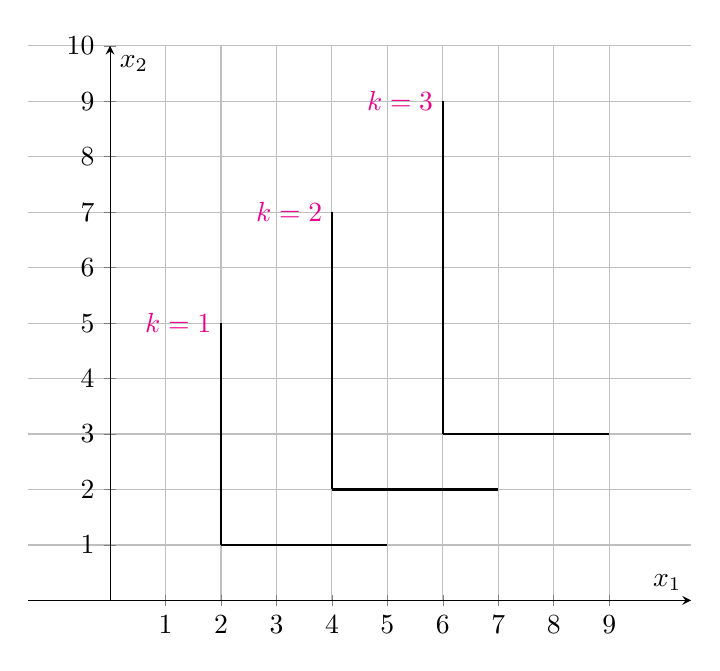
\begin{tikzpicture}[baseline]
              \begin{axis}[axis equal,
                           axis x line = middle,
                           axis y line = middle,
                           grid=both,
                           xmax=9,xmin=0,
                           ymin=0,ymax=10,
                           xlabel=$x_1$,ylabel=$x_2$,
                           xtick={0,...,9},
                           ytick={0,...,10},
                           width=10cm,
                           anchor=center]
                \addplot[thick] coordinates {(2,1)(5,1)};
                \addplot[thick] coordinates {(2,1)(2,5)};
                \draw (2, 5) node [magenta, left] {$k=1$};
                \addplot[thick] coordinates {(4,2)(7,2)};
                \addplot[thick] coordinates {(4,2)(4,7)};
                \draw (4, 7) node [magenta, left] {$k=2$};
                \addplot[thick] coordinates {(6,3)(9,3)};
                \addplot[thick] coordinates {(6,3)(6,9)};
                \draw (6, 9) node [magenta, left] {$k=3$};
              \end{axis}
            \end{tikzpicture}
          \end{center}
        }
      \item What is the marginal rate of substitution when $x_1 = 3$ and
        $x_2=1$? Interpret this number.

        \textcolor{solution-color}{
          When $x_1=3$ and $x_2=1$, we can see that the indifference curve is
          flat and hence its slope is 0. Since the slope of the indifference curve
          at a point is the same as the marginal rate of subsitution at that
          point, we have $MRS=0$. This means that the consumer would be willing
          to give up a small amoumt of $x_1$ in return for zero $x_2$. The
          consumer is willing to throw away some $x_1$ without getting any
          $x_2$ in return.
        }
    \end{itemize}
  \item $u\left( x_1, x_2 \right)=x_1^{\frac{1}{3}}x_2^{\frac{2}{3}}$
    \begin{itemize}
      \item Sketch the indifference curves of the utility function for
        fixed levels of utility $k=1$, $k=2$ and $k=3$.

        \textcolor{solution-color}{
          Setting utility equal to $k$ and solving for $x_2$:
          \begin{align*}
            k&=x_1^{\frac{1}{3}}x_2^{\frac{2}{3}}\\
            x_2^{\frac{2}{3}}&=\frac{k}{x_1^{\frac{1}{3}}}\\
            x_2&=\frac{k^{\frac{3}{2}}}{x_1^{\frac{1}{2}}}\\
          \end{align*}
          Graphing the indifference curves:
          \begin{center}
            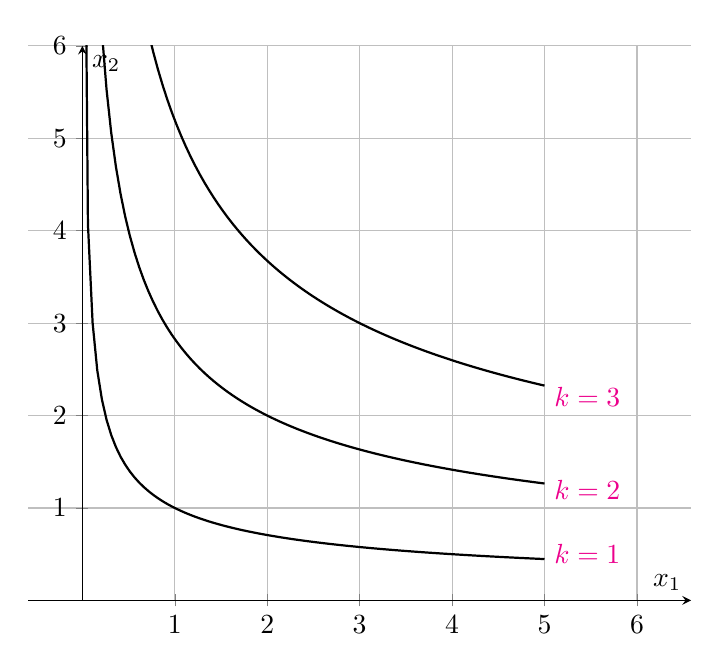
\begin{tikzpicture}[baseline]
              \begin{axis}[axis equal,
                           grid=both,
                           axis x line = middle,
                           axis y line = middle,
                           xmax=6,xmin=0,
                           ymin=0,ymax=6,
                           domain=0.01:5,
                           xlabel=$x_1$,ylabel=$x_2$,
                           xtick={0,...,6},
                           ytick={0,...,6},
                           width=10cm,
                           anchor=center]
                \addplot[thick, samples=100] {1^(3/2) / x^(0.5)};
                \addplot[thick, samples=100] {2^(3/2) / x^(0.5)};
                \addplot[thick, samples=100] {3^(3/2) / x^(0.5)};
                \draw (5, 0.5) node [magenta, right] {$k=1$};
                \draw (5, 1.2) node [magenta, right] {$k=2$};
                \draw (5, 2.2) node [magenta, right] {$k=3$};
              \end{axis}
            \end{tikzpicture}
          \end{center}
        }
      \item Calculate the marginal rate of substitution between the two
        goods.

        \textcolor{solution-color}{
          The marginal utility from $x_1$ is $\frac{\partial u\left( x_1,x_2
          \right)}{\partial x_1}=\frac{1}{3}x_1^{\frac{1}{3}-1}x_2^{\frac{2}{3}}$
          and the marginal utility from $x_2$ is $\frac{\partial u\left( x_1,x_2
          \right)}{\partial x_2}=\frac{2}{3}x_1^{\frac{1}{3}}x_2^{\frac{2}{3}-1}$.
          The marginal rate of substitution is then:
          \[
            MRS=-\frac{\frac{1}{3}x_1^{\frac{1}{3} -
            1}x_2^{\frac{2}{3}}}{\frac{2}{3}x_1^{\frac{1}{3}}x_2^{\frac{2}{3}-1}}=
            -\frac{\frac{1}{3}x_1^{-1}}{\frac{2}{3}x_2^{-1}}=-\frac{x_2}{2x_1}
          \]
        }
    \end{itemize}
\end{subquestions}

\end{document}
